\documentclass[a4paper,danish]{article}
\usepackage[margin=3.5cm]{geometry}

\usepackage[utf8]{inputenc}
\usepackage[T1]{fontenc}
\usepackage{natbib, dsfont, enumitem,
  amssymb,soul,xcolor,amsmath,amsthm,graphicx,subcaption,verbatim,pgfplots,tikz,prodint}
\usetikzlibrary{calc,patterns,angles,quotes,automata,
  positioning,arrows,shapes}

\definecolor{linkcolor}{rgb}{0, 0, 0.54}
\usepackage[colorlinks,allcolors=linkcolor]{hyperref}

\usepackage[author=]{fixme}
\fxusetheme{color}
\definecolor{fxtarget}{rgb}{.5,.5,.5}
\definecolor{fxnote}{rgb}{.5,.5,.5}

\fxsetup{status=draft}

% Ref and bibliography style 
\bibliographystyle{abbrvnat}

% Handling new lines
\setlength{\parskip}{1em}
\setlength{\parindent}{0em}
\usepackage{marginnote}
% Handling space after sections
\usepackage{titlesec}
\titlespacing*{\section}{0em}{2em}{0em}
\titlespacing*{\subsection}{0em}{2em}{0em}
\titlespacing*{\subsubsection}{0em}{2em}{0em}

% No spacing after in start of list
\setlist[itemize]{topsep=0pt}
\setlist[enumerate]{topsep=0pt}

% Theorem environments 
\theoremstyle{plain} % plain italic style
\newtheorem{theorem}{Theorem}
\numberwithin{theorem}{section}
\newtheorem*{theorem*}{Theorem}
\newtheorem{conjecture}{Conjecture}
\newtheorem{lemma}[theorem]{Lemma}
\newtheorem{proposition}[theorem]{Proposition}
\newtheorem{corollary}[theorem]{Corollary}

\theoremstyle{definition} % non-italic
\newtheorem{definition}[theorem]{Definition}
\newtheorem{assumption}[theorem]{Assumption}
\newtheorem*{assumption*}{Assumption}

\theoremstyle{remark}
\newtheorem{remark}[theorem]{Remark}
\newtheorem{example}[theorem]{Example}
\newtheorem{note}[theorem]{Note}

% Notation
\DeclareMathOperator{\E}{\mathbb{E}} % expectation
\newcommand{\Z}{\mathbb{Z}}
\newcommand{\R}{\mathbb{R}}
\newcommand{\N}{\mathbb{N}}
\newcommand{\C}{\mathbb{C}}
\renewcommand{\S}{\mathbb{S}}
\newcommand{\blank}{\makebox[1ex]{\textbf{$\cdot$}}}
\newcommand\independent{\protect\mathpalette{\protect\independenT}{\perp}}
\def\independenT#1#2{\mathrel{\rlap{$#1#2$}\mkern2mu{#1#2}}}
\renewcommand{\phi}{\varphi}
\renewcommand{\epsilon}{\varepsilon}
\newcommand*\diff{\mathop{}\!\mathrm{d}}
\newcommand{\weakly}{\rightsquigarrow}
\newcommand\smallO{\textit{o}}
\newcommand\bigO{\textit{O}}
\newcommand{\midd}{\; \middle|\;}
\newcommand{\1}{\mathds{1}}
\usepackage{ifthen} %% Empirical process with default argument
\newcommand{\G}[2][n]{
{\ensuremath{\mathbb{G}_{#1}}{\left[#2\right]}}
}
\DeclareMathOperator*{\argmin}{\arg\!\min}
\DeclareMathOperator*{\argmax}{\arg\!\max}
\newcommand{\empmeas}{\ensuremath{\mathbb{P}_n}} % empirical measure
\newcommand{\data}{\ensuremath{\mathcal{D}}}



\title{The Joint Survival Super Learner: A super learner for right-censored
  data}
\author{Anders Munch \& Thomas A. Gerds}
\date{\today}

\begin{document}
\maketitle


\begin{abstract} Risk prediction models are widely used to guide
real-world decision-making in areas such as healthcare and economics,
and they also play a key role in estimating nuisance parameters in
semiparametric inference. The super learner is a machine learning
framework that combines a library of prediction algorithms into a
meta-learner using cross-validated loss. In the context of
right-censored data, careful consideration must be given to both the
choice of loss function and the estimation of expected loss. Moreover,
estimators such as inverse probability of censoring weighting (IPCW)
require accurate modeling and estimates of the censoring distribution.

We propose a novel approach to super learning for survival analysis
that jointly evaluates candidate learners for both the event time
distribution and the censoring distribution. Our method imposes no
restrictions on the algorithms included in the library, accommodates
competing risks, and does not rely on a single pre-specified estimator
of the censoring distribution. We establish an oracle inequality for
our method, assess its performance through simulation studies, and
demonstrate its practical utility using prostate cancer data.
\end{abstract}

\textit{\textbf{Keywords:} Competing risks, cross-validation,
  loss based estimation, right-censored data, super learner}

\section{Introduction}
\label{sec:introduction}

Accurately predicting risk from time-to-event data is a central
challenge in diverse research fields including epidemiology, economics
and weather forecasting with applications in clinical
decision making and policy interventions. For instance, in prostate
cancer management, clinicians often need to estimate a patient’s risk
of disease progression and mortality over time to make informed
decisions about treatment strategies such as active surveillance
versus immediate intervention. Reliable time-to-event risk predictions
can help tailor care to individual patients, avoid overtreatment, and
allocate healthcare resources more effectively. Super learning
\citep{van2007super}, also known as ensemble learning or stacked
regression \citep{wolpert1992stacked,breiman1996stacked}, provides a
powerful approach to this problem by combining multiple
candidate prediction models to reduce the risk of bias incurred by a
single potentially mispecified model. In survival analysis, a super
learner may combine a stack of Cox regression models with a stack of
random survival forests \citep[][Section 8.4]{gerds2021medical}. Such
a strategy has recently produced KDpredict
(\url{https://kdpredict.com/}) a model which jointly predicts the
risks of kidney failure and all-cause mortality at multiple time
horizons based on different sets of covariates
\citep{liu2024predicting}. To evaluate the prediction performance of
the learners the super learner behind KDpredict uses inverse
probability of censoring weighting (IPCW) where the censoring
distribution is estimated under the restrictive assumption that the
censoring distribution does not depend on the covariates. This is a
potential source of bias which is difficult to overcome with the
currently available methods.


In this paper we propose the Joint Survival Super Learner (JSSL), a
new super learner designed to handle the specific challenges of
ensemble learning with right-censored data. The JSSL jointly
learns prediction models for the event-time and censoring
distributions. The JSSL is based on the simple idea of an
artificial competing risk model where censoring is included as a state
of its own. Candidate learners of the event time hazard and censoring
hazard functions are then assessed based on how well they predict the
state occupation probabilities of the artificial competing risk model
across time based on baseline covariate information. Our estimation
framework allows for competing risks, avoids restrictive assumptions
on the censoring distribution, and is also fully flexible with respect
to the choice of learners. The latter is in contrast to other
proposals which restrict the library of learners to specific model
classes \citep{polley2011-sl-cens,golmakani2020super}, see Section
\ref{sec:choice-of-loss-function}. Like our proposal, recent work by
\cite{han2021inverse} and \cite{westling2021inference} also
circumvents the need to pre-specify a censoring model by iterating
between estimation of the outcome and censoring models. However, this
iterative procedure is in general not guaranteed to converge to the
true data-generating mechanism
\citep[][Appendix~A.4]{munch2024thesis}.

To analyse the theoretical properties of JSSL we
focus on the discrete super learner which picks the model in
the library with best estimated performance
\citep{van2007super}. We provide theoretical guarantees
for the performance of JSSL and in particular
show that discrete JSSL is consistent under
natural conditions and prove a finite-sample oracle
inequality. We demonstrate how to construct a library for JSSL using common survival models, and how to obtain
risk predictions from the resulting ensemble.

The rest of the paper is organized as follows.
We introduce our notation and framework in
Section~\ref{sec:framework}. Section~\ref{sec:super-learning}
introduces loss-based super learning. In
Section~\ref{sec:super-learner-simple} we define JSSL,
while Section~\ref{sec:theor-results-prop} provides theoretical
guarantees. In Section~\ref{sec:use-cases-state} we demonstrate how
JSSL can be used to obtain risk predictions, and we
briefly mention how it can be applied in the context of causal
inference.  Section~\ref{sec:numer-exper} reports the results of
numerical experiments, and Section~\ref{sec:real-data-appl}
illustrates the method on prostate cancer data. We conclude with a
discussion in Section~\ref{sec:discussion}. Proofs are collected in
Appendix~\ref{sec:proofs}. Code and an implementation of JSSL are available at \url{https://github.com/amnudn/statelearner}.

\section{Notation and framework}
\label{sec:framework}

In a competing risk framework \citep{andersen2012statistical}, let \(
T\) be a time to event variable, \(D\in\{1,2\}\) the cause of the
event, and $X \in \mathcal{X}$ a vector of baseline covariates taking
values in a bounded subset \( \mathcal{X} \subset \R^p \), \( p\in\N
\). Let $\tau< \infty$ be a fixed prediction horizon. We use \(
\mathcal{Q} \) to denote the collection of all probability measures on
\( [0,\tau] \times \{1,2\}\times \mathcal{X} \) such that \( (T, D, X)
\sim Q \) for some unknown \( Q \in \mathcal{Q} \). For
\(j\in\{1,2\}\), the cause-specific conditional cumulative hazard
functions \( \Lambda_{j} \colon [0, \tau] \times \mathcal{X}
\rightarrow \R_+ \) are defined as
\begin{equation*}
  % \label{eq:cum-haz}
  \Lambda_{j}(t \mid x) = \int_0^t\frac{  Q(T \in \diff s, D=j \mid X=x )}{Q(T \geq s \mid X=x )}.
\end{equation*} For ease of presentation we assume throughout that the
map \( t\mapsto \Lambda_j(t \mid x) \) is continuous for all \( x \)
and \( j \), however, 
all technical arguments extend naturally to the general case \citep{andersen2012statistical}.
The event-free survival function conditional on covariates is given by
\begin{equation}
  \label{eq:surv-def}
  S(t \mid x)=\exp\left\{-\Lambda_{1}(t \mid x)-\Lambda_{2}(t \mid x)\right\}.
\end{equation}
Let \( \mathcal{M}_{\tau}\) denote the space of all conditional cumulative hazard
functions on \( [0,\tau] \times\mathcal{X}\). Any distribution
\( Q \in \mathcal{Q} \) can be characterised by
\begin{equation*}
  \label{eq:parametrizeQ}
  \begin{split}
    Q(\diff t,j,\diff x)=& \left\{S(t- \mid x)\Lambda_1(\diff t \mid x)H(\diff x)\right\}^{\1{\{j=1\}}}\\
                         &  \left\{S(t- \mid x)\Lambda_2(\diff t \mid x)H(\diff x)\right\}^{\1{\{j=2\}}},
  \end{split}
\end{equation*}
where \(\Lambda_{j} \in \mathcal{M}_{\tau}\) for \(j=1,2\) and \(H\) is the marginal
distribution of the covariates.

We consider the right-censored setting in which we observe \(O =
(\tilde{T},\tilde D, X)\), where $\tilde T = \min(T,C)$ for a
right-censoring time \(C\), $\Delta = \1{\{T \leq C\}}$, and \(\tilde
D=\Delta D\). Let \(\mathcal{P}\) denote a set of probability measures
on the sample space \(\mathcal{O} = [0, \tau] \times \{0, 1, 2\}
\times \mathcal{X}\) such that \(O \sim P \) for some unknown \(P\in
\mathcal{P}\). We assume that the event times and the censoring times
are conditionally independent given covariates, \( T \independent C
\mid X \). This implies that any distribution \( P \in \mathcal{P} \)
is characterised by a distribution \( Q \in \mathcal{Q} \) and a
conditional cumulative hazard function for \( C \) given \( X \)
\citep[c.f.,][]{begun1983information,gill1997coarsening}. We use
\(\Gamma\in\mathcal{M}_{\tau}\) to denote the cumulative hazard
function of the conditional censoring distribution given
covariates. For ease of presentation we assume that \(t\mapsto
\Gamma(t \mid x) \) is continuous for all \( x \). We let
\((t,x)\mapsto G(t \mid x)=\exp\left\{-\Gamma(t \mid x)\right\}\)
denote the survival function of the conditional censoring
distribution. The distribution \( P \) is characterised by
\begin{equation}\label{eq:parametrizeP}
  \begin{split}
    P(\diff t, j, \diff x) =& \left\{G(t- \mid x)S(t- \mid x)\Lambda_1(\diff t \mid x)H(\diff x)\right\}^{\1{{\{j=1\}}}}\\
                            & \left\{G(t- \mid x)S(t- \mid x)\Lambda_2(\diff t \mid x)H(\diff x)\right\}^{\1{{\{j=2\}}}}\\
                            & \left\{G(t- \mid x)S(t- \mid x)\Gamma(\diff t \mid x)H(\diff x)\right\}^{\1{{\{j=0\}}}}\\
    = & \left\{G(t- \mid x)Q(\diff t,j,\diff x)\right\}^{\1{{\{j\ne 0\}}}}\\    
                            & \left\{G(t- \mid x)S(t- \mid x)\Gamma(\diff t \mid x)H(\diff x)\right\}^{\1{{\{j=0\}}}}.
  \end{split}
\end{equation}
Hence, we may write
\( \mathcal{P} = \{ P_{Q, \Gamma} : Q \in \mathcal{Q}, \Gamma \in
\mathcal{G} \} \) for some \( \mathcal{G} \subset \mathcal{M}_{\tau} \). We
also have \(H\)-almost everywhere
\begin{equation*}
P(\tilde T>t \mid X=x) = S(t \mid x)G(t \mid x) = \exp\left\{-\Lambda_{1}(t \mid x)-\Lambda_{2}(t \mid x)-\Gamma(t \mid x) \right\}.
\end{equation*} We assume that there exists \(\kappa<\infty\) such
that \(\Lambda_{j}(\tau- \mid x)<\kappa \), for \(j\in\{1,2\}\), and
\(\Gamma(\tau- \mid x)<\kappa\) for almost all \(x\in\mathcal
X\). Note that this implies that \(G(\tau- \mid x)\) is bounded away
from zero for almost all \(x\in\mathcal X\).  Under these assumptions,
the conditional cumulative hazard functions \(\Lambda_{j}\) and
\(\Gamma\) can be identified from \(P\) by
\begin{align}
  \Lambda_{j}(t \mid x) &= \int_0^t\frac{  P(\tilde T \in \diff s, \tilde D=j \mid X=x )}{P(\tilde T \geq s \mid X=x )}, \label{eq:lambdaj}\\
  \Gamma(t \mid x) &= \int_0^t\frac{  P(\tilde T \in \diff s, \tilde D=0 \mid X=x )}{P(\tilde T \geq s \mid X=x )}\label{eq:gamma}.
\end{align}
Thus, we can consider $\Lambda_j$ and \(\Gamma\) as operators which map from
\( \mathcal{P} \) to \(\mathcal M_{\tau}\).

\section{Loss-based super learning}
\label{sec:super-learning}

Loss-based super learning requires a library of candidate models, or
\textit{learners}, a cross-validation algorithm, and a loss function
for evaluating prediction performance on hold-out samples. In this
section we provide an abstract definition of loss-based super
learning. As input to a super learner we need a data set
\( \data_n=\{O_i\}_{i=1}^n \) of i.i.d.\ observations from
\( P \in \mathcal{P} \) and a collection of candidate models or
learners $\mathcal{A}$. Let \(\Theta\) be a suitable parameter space,
which will in our case be a class of functions representing different
models. Each learner
\(a \in \mathcal{A}\) is a map
\( a \colon \mathcal{O}^n \rightarrow \Theta \) which takes a data set
as input and returns an estimate $a(\data_n)$ of $\theta$. Let
\(L\colon \Theta \times \mathcal{O} \rightarrow \R_+\) be a loss
function, representing the performance of the model
$\theta \in \Theta$ at the observation \( O \in \mathcal{O} \), where
lower values mean better performance.

The expected
loss of a learner is estimated by splitting the data set $\data_n$
into $K$ disjoint approximately equally sized subsets
\(\data_n^1, \data_n^2, \dots, \data_n^K \) and then calculating the
cross-validated loss
\begin{equation*}
  % \label{eq:cv-risk-est}
  \hat{R}_n(a; L) =
  \frac{1}{K}\sum_{k=1}^{K}
  % \empmeas^k{[L {(a{ (\data_n^{-k})} , \blank) }]},
  \frac{1}{| \data_n^{k} |}\sum_{O_i \in \data_n^{k}}
  L
  {
    \left(
      a{ (\data_n^{-k})}
      , O_i
    \right)
  },
  \quad \text{with} \quad
  \data_n^{-k} = \data_n \setminus \data_n^{k}.
\end{equation*}
% where \( \empmeas^{k} \) is the empirical measure of \( \data_n^{k} \). 
The subset \(\data_n^{-k}\) is referred to as the \(k\)'th training
sample, while \(\data_n^{k}\) is referred to as the \(k\)'th test or
hold-out sample.
The discrete super learner is defined as
\begin{equation*}
\hat{a}_n = \argmin_{a\in\mathcal A}\hat{R}_n(a; L).
\end{equation*}
The oracle learner is defined as the learner that minimises the
expected loss under the data-generating distribution \( P \),
i.e.,
\begin{equation*}
  \tilde{a}_n =
  \argmin_{a \in \mathcal{A}}
  \tilde{R}_n(a; L),
  \quad \text{with} \quad 
  \tilde{R}_n(a; L)=
  \frac{1}{K}\sum_{k=1}^{K} 
  P{
    \left[
      L
      {
        \left(
          a{ (\data_n^{-k})}
          , \blank
        \right)
      }
    \right]}
  .
\end{equation*}
Note that both the discrete super learner and the oracle learner
depend on the library of learners and on the number of folds \(K\),
and that the oracle learner is a function of the data and the unknown
data-generating distribution.
% However, these dependencies are suppressed in the notation.

\section{The joint survival super learner (JSSL)}
\label{sec:super-learner-simple}

The main idea of JSSL is to jointly use learners for \(
\Lambda_1 \), \( \Lambda_2 \), and \( \Gamma \), and the relations in
equation~(\ref{eq:parametrizeP}), to learn a feature of the observed
data distribution \( P \). Discrete JSSL ranks a tuple of
learners for the tuple of the cumulative hazard functions \(
(\Lambda_1, \Lambda_2, \Gamma) \) based on how well they jointly model
the observed data. To formally introduce JSSL, we define
the process 
\begin{equation*}
  \eta(t) = \1\{\tilde{T} \leq t, \tilde D=1\} + 2\,\1\{\tilde{T} \leq t, \tilde
  D=2\} - \1\{\tilde{T} \leq t, \tilde D=0\},
  \quad \text{for} \quad t \in [0, \tau],
\end{equation*}
which takes values in \( \{-1,0,1,2\}\). The four values
represent four mutually exclusive states. Specifically, value
\( 0 \) represents the state where the individual is still
event-free and uncensored, value \( 1\) the state where the
event of interest has occurred, value \( 2\) the state where a
competing risk has occurred, and value \( -1\) the state where
the observation is right-censored. The state occupation
probabilities given baseline covariates \( X \) are given by
the function
\begin{equation}
  \label{eq:F-def}
  F(t, l, x) = P(\eta(t) = l \mid X=x),
\end{equation}
for all \( t \in [0,\tau] \), \( l \in \{-1,0,1,2\} \), and
\( x \in \mathcal{X} \).

The JSSL is a super learner for the function-valued parameter
$\theta(P) = F$ which is identified through
equation~(\ref{eq:F-def}). Under conditional independent censoring
each tuple $(\Lambda_{1}, \Lambda_{2}, \Gamma, H)$ characterises a
distribution \(P\in\mathcal P\), c.f.\
equation~\eqref{eq:parametrizeP}, which in turn determines \( (F, H)
\). Hence, a learner for \( F \) can be constructed from learners for
\( \Lambda_1 \), \( \Lambda_2 \), and $\Gamma$ as follows:
\begin{equation}\label{eq:transition}
  \begin{split}
    F(t, 0, x)
    &
      = P(\tilde{T} > t \mid X= x)
      =
      \exp{{\{-\Lambda_{1}(t \mid x)-\Lambda_{2}(t \mid x) - \Gamma(t \mid x)\}
      }},
    \\
    F(t, 1, x)
    &
      = P(\tilde{T} \leq t, \tilde{D}=1 \mid X=x)
      = \int_0^t F(s-, 0, x)  \Lambda_{1}(\diff s \mid x),
    \\
    F(t, 2, x)
    &
      = P(\tilde{T} \leq t, \tilde{D}=2 \mid X=x)
      = \int_0^t  F(s-, 0, x)  \Lambda_{2}(\diff s \mid x),
    \\
    F(t, -1, x)
    &
      = P(\tilde{T} \leq t, \tilde{D}=0 \mid X=x)
      = \int_0^t F(s-, 0, x)  \Gamma(\diff s \mid x).
  \end{split}
\end{equation}
Equation~\eqref{eq:transition} implies that a library for JSSL can by build from three libraries of learners:
\(\mathcal{A}_1\), \( \mathcal{A}_2 \), and \( \mathcal{B} \),
where \(\mathcal{A}_1\) and \( \mathcal{A}_2\) contain
learners for the conditional cause-specific cumulative hazard
functions \(\Lambda_1\) and \( \Lambda_2\), respectively, and
\(\mathcal{B}\) contains learners for the conditional
cumulative hazard function of the censoring distribution.
Based on the Cartesian product of libraries of learners for
\((\Lambda_1,\Lambda_2,\Gamma)\) we construct a library
$\mathcal{F}$ of learners for \( F \):
\begin{align*}
  \mathcal{F}(\mathcal{A}_1, \mathcal{A}_2, \mathcal{B})
  &= \{ \phi_{a_1,a_2, b} : a_1 \in \mathcal{A}_1, a_2 \in \mathcal{A}_2, b \in \mathcal{B}\},
    \intertext{where in correspondence with  the relations in equation
    \eqref{eq:transition},}
    \phi_{a_1,a_2, b}(\data_n)(t,0,x)
  &= \exp{\{-a_1(\data_n)(s \mid x)-a_2(\data_n)(s \mid x) - b(\data_n)(s \mid
    x)\} },
  \\
  \phi_{a_1,a_2, b}(\data_n)(t,1,x)
  &= \int_0^t
    \phi_{a_1,a_2, b}(\data_n)(s-,0,x)  a_1(\data_n)(\diff s \mid x),
  \\
  \phi_{a_1,a_2, b}(\data_n)(t,2,x)
  &= \int_0^t\phi_{a_1,a_2, b}(\data_n)(s-,0,x)  a_2(\data_n)(\diff s \mid x),
  \\
  \phi_{a_1,a_2, b}(\data_n)(t,-1,x)
  &= \int_0^t \phi_{a_1,a_2, b}(\data_n)(s-,0,x)  b(\data_n)(\diff s \mid x).
\end{align*} Notably, the libraries \( \mathcal{A}_1 \), \(
\mathcal{A}_2 \), and \( \mathcal{B} \) can be constructed using
standard software for survival analysis. In
\texttt{R}, for instance, we can construct Cox models as
learners using the \texttt{survival}-package
\citep{survival-package}, and we can construct random survival
forests as learners using the \texttt{randomForestSRC}-package \citep{randomForestSRC}.

To evaluate how well a function \( F \) predicts the
process $\eta$ we use the integrated Brier score \citep{graf1999assessment}
\( \bar B_\tau( F,O) = \int_0^{\tau} B_t(F,O) \diff t \),
where \( B_t \) is the Brier score
\citep{brier1950verification} at time \( t \in [0, \tau] \),
\begin{equation*}
  B_t(F,O) = \sum_{l=-1}^{2}
  \left(
      F(t,l,X) - \1{\{\eta(t)=l\}}
  \right)^2.
\end{equation*}
\marginnote{Say that Brier score is across all 4 states because this is not commonly done}
Based on a split of a data set \(\data_n\) into $K$ disjoint
approximately equally sized subsets (c.f., Section
\ref{sec:super-learning}), each learner
\( \phi_{a_1, a_2, b} \) in the library
\( \mathcal{F}(\mathcal{A}_1, \mathcal{A}_2, \mathcal{B}) \)
is evaluated using the cross-validated loss,
\begin{equation*}
  \hat{R}_{n}(\phi_{a_1,a_2,b} ; \bar{B}_{\tau}) =
  \frac{1}{K}\sum_{k=1}^{K}
  \frac{1}{| \data_n^{k} |}\sum_{O_i \in \data_n^{k}}
  \bar B_\tau
  {
    \left(
      \phi_{a_1,a_2,b}{ (\data_n^{-k})}
      , O_i
    \right)
  },
\end{equation*}
and discrete JSSL is given by
\begin{align*}\label{eq:discrete-state-learner}
  \hat{\phi}_n
  &=  \argmin_{(a_1,a_2,b)\in \mathcal{A}_1\times\mathcal{A}_2\times\mathcal{B}}
    \hat{R}_{n}(\phi_{a_1,a_2,b} ; \bar{B}_{\tau}).
\end{align*}




\section{Theoretical guarantees}
\label{sec:theor-results-prop}

\marginnote{depending on the journal both subsections may benefit from explanations about the usefulness of these results} 
In this section we show that JSSL is consistent if its
library contains a consistent learner, and we establish a finite
sample inequality for the excess risk of JSSL compared to
the oracle.

\subsection{Consistency}
\label{sec:consistency}

% We let \( \E_P \) denote
% expectation under \( P \) and use \( \Theta \) to denote the
% collection of all conditional state-occupation probability functions.
The following result can be derived from the fact
that the integrated Brier score (also called the continuous
ranked probability score) is a strictly proper scoring rule
\citep{gneiting2007strictly}. This implies that if we minimise
the average loss of the integrated Brier score, we recover the
parameters of the data-generating distribution. Specifically,
this implies that the oracle of a JSSL is consistent
if the library of learners contains at least one learner that
is consistent for estimation of \( F \). Recall that the
function \(F\) implicitly depends on the data-generating
probability measure \(P\in\mathcal P\) but that this was
suppressed in the notation. We now make this dependence
explicit by writing \(F_P\) for the function determined by a
given \(P \in\mathcal{P}\) in accordance with equation
equation~(\ref{eq:F-def}). In the following we let
\( \mathcal{H}_{\mathcal{P}} = \{F_P : P \in \mathcal{P}\} \).

\begin{proposition}
  \label{prop:stric-prop}
  If \(P \in\mathcal{P}\) then
  \begin{equation*}
    F_P = \argmin_{F \in \mathcal{H}_{\mathcal{P}}} P{[\bar{B}_\tau(F, \blank)]},
  \end{equation*}
  for all \( l \in \{-1, 0, 1, 2 \} \), almost all
  \( t \in [0,\tau] \), and \( P \)-almost all
  \( x \in \mathcal{X} \).
\end{proposition}
\begin{proof}
  See Appendix~\ref{sec:consistency-proof}.
\end{proof}

\subsection{Oracle inequality}
\label{sec:finite-sample-oracle}

To establish a finite sample oracle result for JSSL we
assume a split of the data into equally sized folds, and for
simplicity of presentation we take \( n \) to be such that \(
|\data_n^{-k}| = n/K \) with \( K \) fixed. We will allow the number
of learners to grow with \( n \) and write \(
\mathcal{F}_n=\mathcal{F}(\mathcal{A}_{1,n}, \mathcal{A}_{2,n},
\mathcal{B}_n)\) as short-hand notation emphasing the
dependence on the sample size. In the following we let the space \(
\mathcal{H}_{\mathcal{P}}= \{F_P : P \in \mathcal{P}\} \) be equipped with the norm \( \| \blank
\|_{P} \) defined by
\begin{equation}
  \label{eq:norm}
  \| F \|_{P} = 
  \left\{
    \sum_{l=-1}^{2}\int_{\mathcal{X}} \int_0^{\tau} F(t, l, x)^2 \diff t P( \diff x)
  \right\}^{1/2}.
\end{equation}

\begin{proposition}
  \label{prop:oracle-prop}
  For all \(P\in\mathcal{P}\), \( n \in \N \), \( k \in \{1, \dots, K\} \),
  and $\delta>0$,
  \begin{align*}
    \E_{P}{\left[ \Vert \hat{\phi}_n(\data_n^{-k}) - F_P \Vert_{P}^2 \right]}
    & \leq (1 + 2\delta)
      \E_{P}{\left[ \Vert \tilde{\phi}_n(\data_n^{-k}) - F_P \Vert_{P}^2 \right]}
    \\
    & \quad
      + (1+ \delta) 16   K \tau
      \left(
      13 + \frac{12}{\delta}
      \right)
      \frac{\log(1 + |\mathcal{F}_n|)}{n}.
  \end{align*}
\end{proposition}
\begin{proof}
  See Appendix~\ref{sec:oracle-inequalities}.
\end{proof}

Proposition~\ref{prop:oracle-prop} has the following
asymptotic consequences.

\begin{corollary}
  \label{cor:asymp-cons}
  Assume that \( |\mathcal{F}_n| = \bigO(n^q)\), for some \( q \in \N \) and
  that there exists a sequence \( \phi_n \in \mathcal{F}_n \), \( n \in \N \),
  such that
  \( \E_{P}{\left[ \Vert \phi_n(\data_n^{-k}) - F_P \Vert_{P}^2 \right]} =
  \bigO(n^{-\alpha}) \), for some \( \alpha\leq 1 \).
  \begin{enumerate}[label=(\alph*)]
  \item If $\alpha=1$ then
    \( \E_{P}{\left[ \Vert \hat{\phi}_n(\data_n^{-k}) - F_P \Vert_{P}^2
      \right]} = \bigO(\log(n)n^{-1}) \).
  \item If $\alpha<1$ then
    \( \E_{P}{\left[ \Vert \hat{\phi}_n(\data_n^{-k}) - F_P \Vert_{P}^2 \right]} =
    \bigO(n^{-\alpha}) \).
  \end{enumerate}
\end{corollary}
\begin{proof}
  See Appendix~\ref{sec:oracle-inequalities}.
\end{proof}

Proposition~\ref{prop:oracle-prop} provides a bound on the
average price we pay for using cross-validation to select a
learner from a library of candidates as compared to knowing
the oracle learner in advance. Corollary~\ref{cor:asymp-cons}
states that this price is asymptotically vanishing, up to
logarithmic terms, as long as the number of learners in the
library grows with sample size at a polynomial rate.

\section{Use cases for JSSL}
\label{sec:use-cases-state}
\marginnote{both subsections would benefit from examples. could we merge with section 8?} 
The JSSL estimates the function \( F \) which depends on the
censoring distribution and is typically not of direct interest in
itself. In the following, we describe how an estimate of \( F \), as
provided by JSSL, can be used to predict risks over time.

\subsection{Survival and risk predictions}
\label{sec:surv-risk-pred}

Event-free survival probabilities and risk predictions can be
obtained from the state-occupation function \( F \) under the
assumption of conditional independent censoring and
positivity, as introduced in Section~\ref{sec:framework}. By
equations~(\ref{eq:lambdaj}) and~(\ref{eq:gamma}) and the
definition of \( F \), we have
\begin{equation}
  \label{eq:7}
  % \Gamma(t , x) = \int_0^t \frac{F(\diff s, -1, x )}{F(s-,
  % 0, x )}, \quad \text{and} \quad
  \Lambda_j(t , x) 
  = \int_0^t  \frac{F(\diff s, j, x )}{F(s-, 0, x )},
  \quad j \in \{1,2\}.
\end{equation}
Equation~\eqref{eq:surv-def} provides a formula for obtaining
event-free survival probabilities from the cause-specific
cumulative hazard functions. Similarly, cause-specific risk
predictions can be obtained from \( \Lambda_1 \) and
$\Lambda_2$ using the formula
\citep[e.g.,][]{benichou1990estimates,
  ozenne2017riskregression},
\begin{equation}
  \label{eq:cs-risk-def}
  Q(T \leq t, D = j \mid X=x) =
  \int_0^t \exp\left\{-\Lambda_{1}(u \mid x)-\Lambda_{2}(u
    \mid x)\right\}  \Lambda_j(\diff u \mid x),
  \quad j \in \{1,2\}.
\end{equation}
Hence, given JSSL's estimate of \( F \) we can
use equation~\eqref{eq:7} to obtain estimates of the
cause-specific cumulative hazard functions $\Lambda_j$, which
can in turn be used to obtain estimates of the event-free
survival probabilites and cause-specific risks through
equations~\eqref{eq:surv-def} and~\eqref{eq:cs-risk-def}.

In Section~\ref{sec:super-learner-simple} we suggested to
implement JSSL by building a library using
learners of the cause-specific cumulative hazard functions,
$\Lambda_j$, and the cumulative hazard function for censoring,
$\Gamma$. With this implementation we can directly input the
highest ranked tuple of cause-specific hazard functions
$(\Lambda_1, \Lambda_2)$ provided by JSSL as
input to equations~\eqref{eq:surv-def}
and~\eqref{eq:cs-risk-def}.

\subsection{Targeted machine learning and causal inference}
\label{sec:targeted-learning}

The framework of \textit{targeted} or \textit{debiased}
machine learning is a general methodology for combining
data-adaptive modeling, such as machine and super learning,
with asymptotically valid statistical inference for
interpretable target parameters \citep{van2006targeted,
  chernozhukov2018double}. \fxnote*{add more references?}{This
  framework has been applied extensively for causal inference
  based on observational data
  \citep[e.g.,][]{van2011targeted,kennedy2016semiparametric,rytgaard2022targeted}.}
A targeted or debiased estimator is constructed by first
estimation high-dimensional nuisance parameters using machine
learning, and then employing a debiasing or targeting step
that is motivated from semi-parametric efficiency theory
\citep{pfanzagl1985contributions,bickel1993efficient,van2003unified,tsiatis2007semiparametric,kennedy2022semiparametric}.
In the context of right-censored competing risk data, the
high-dimensional nuisance parameters needed to be estimated
will typically include the cause-specific cumulative hazard
functions and the cumulative hazard function for censoring
\citep[e.g.,][]{van2003unified,rytgaard2021estimation,rytgaard2022targeted}.
The JSSL immediately provides estimates of these
nuisance parameters and is hence particularly well suited for
targeted and debiased machine learning. Though it served as
our original motivation for developing JSSL, we
leave the study of JSSL in the context of
targeted and debiased machine learning for a future paper.



\section{Numerical experiments}
\label{sec:numer-exper}


In this section we report results from a simulation study where we consider
estimation of the conditional survival function. In the first part, we compare
JSSL to two IPCW based discrete super learners that use either the
Kaplan-Meier estimator or a Cox model to estimate the censoring probability
\citep{gonzalez2021stacked}. In the second part we compare JSSL to
the super learner proposed by \cite{westling2021inference}.

In both parts we use the same data-generating mechanism. We generate data
according to a distribution motivated from a real data set in which censoring
depends on the baseline covariates. We simulate data based on the prostate
cancer study of \cite{kattan2000pretreatment}. The outcome of interest is the
time to tumor recurrence, and five baseline covariates are used to predict
outcome: prostate-specific antigen (PSA, ng/mL), Gleason score sum (GSS, values
between 6 and 10), radiation dose (RD), hormone therapy (HT, yes/no) and
clinical stage (CS, six values). The study was designed such that a patient's
radiation dose depended on when the patient entered the study
\citep{gerds2013estimating}. This in turn implies that the time of censoring
depends on the radiation dose. The data were re-analysed in
\citep{gerds2013estimating} where a sensitivity analysis was conducted based on
simulated data. Here we use the same simulation setup, where event and censoring
times are generated according to parametric Cox-Weibull models estimated from
the original data, and the covariates are generated according to either marginal
Gaussian normal or binomial distributions estimated from the original data
\citep[c.f.,][Section~4.6]{gerds2013estimating}. We refer to this simulation
setting as `dependent censoring'. We also considered a simulation setting where
data were generated in the same way, except that censoring was generated
completely independently. We refer to this simulation setting as `independent
censoring'.

For all super learners we use a library consisting of three
learners: The Kaplan-Meier estimator
\citep{kaplan1958nonparametric,Gerds_2019prodlim}, a Cox model
with main effects \citep{cox1972regression, survival-package},
and a random survival forest
\citep{ishwaran2008random,randomForestSRC}. We use the same
library to learn the outcome distribution and the censoring
distribution. Note that the three learners in our library of
learners can be used to learn the cumulative hazard functions
of the outcome and the censoring distribution. The latter
works by training the learner on the data set \( \data_n^c \),
where \( \data_n^c = \{O_i^c\}_{i=1}^n \) with
\( O_i^c = (\tilde{T}_i, 1-\Delta_i, X_i) \). When we say that
we use a learner for the cumulative hazard function of the
outcome to learn the cumulative hazard function of the
censoring time, we mean that the learner is trained on
\( \data_n^c \).

We compare JSSL to two IPCW based super learners: The
first super learner, called IPCW(Cox), uses a Cox model with main
effects to estimate the censoring probabilities, while the second
super learner, called IPCW(KM), uses the Kaplan-Meier estimator to
estimate the censoring probabilities. The Cox model for the censoring
distribution is correctly specified in both simulation settings while
the Kaplan Meier estimator only estimates the censoring model
correctly in the simulation setting where censoring is
independent. Both IPCW super learners are fitted using the
\texttt{R}-package \texttt{riskRegression}
\citep{Gerds_Ohlendorff_Ozenne_2023}.
%
% | time | sim_setting | true_events | true_cens | at_risk |
% |------+-------------+-------------+-----------+---------|
% |   36 | original    |      24.619 |    61.853 |  25.774 |
% |   36 | indep_cens  |      24.674 |    38.740 |  46.141 |
%
The IPCW super learners use the integrated Brier score up to a fixed time
horizon (36 months). The marginal risk of the event before this time horizon is
\(\approx 24.6\)\%. Under the `dependent censoring' setting the marginal
censoring probability before the time horizon is \(\approx 61.9\)\%. Under the
`independent censoring' setting the marginal censoring probability before this
time horizon is \( \approx 38.7 \)\%.

Each super learner provides a learner for the cumulative
hazard function for the outcome of interest. From the
cumulative hazard function a risk prediction model can be
obtained as described in Section~\ref{sec:surv-risk-pred}
(with the special case of $\Lambda_2 = 0$). We measure the
performance of each super learner by calculating the index of
prediction accuracy (IPA) \citep{kattan2018index} at a fixed
time horizon (36 months) for the risk prediction model
provided by the super learner. The IPA is 1 minus the ratio
between the model's Brier score and the null model's Brier
score, where the null model is the model that does not use any
covariate information. The IPA is approximated using a large
(\( n = 20,000 \)) independent data set of uncensored data. As
a benchmark we calculate the performance of the risk
prediction model chosen by the oracle selector, which uses the
large data set of uncensored event times to select the learner
with the highest IPA.

The results are shown in Figure~\ref{fig:ipcw-fail}. We see that in
the scenario where censoring depends on the covariates, using the
Kaplan-Meier estimator to estimate the censoring probabilities
provides a risk prediction model with an IPA that is lower than the
risk prediction model provided by JSSL. The performance
of the risk prediction model selected by JSSL is similar
to the risk prediction model selected by the IPCW(Cox) super learner
which a priori uses a correctly specified model for the censoring
distribution. Both these risk prediction models are close to the
performance of the oracle, except for small sample sizes.

\begin{figure}
  \centering %
  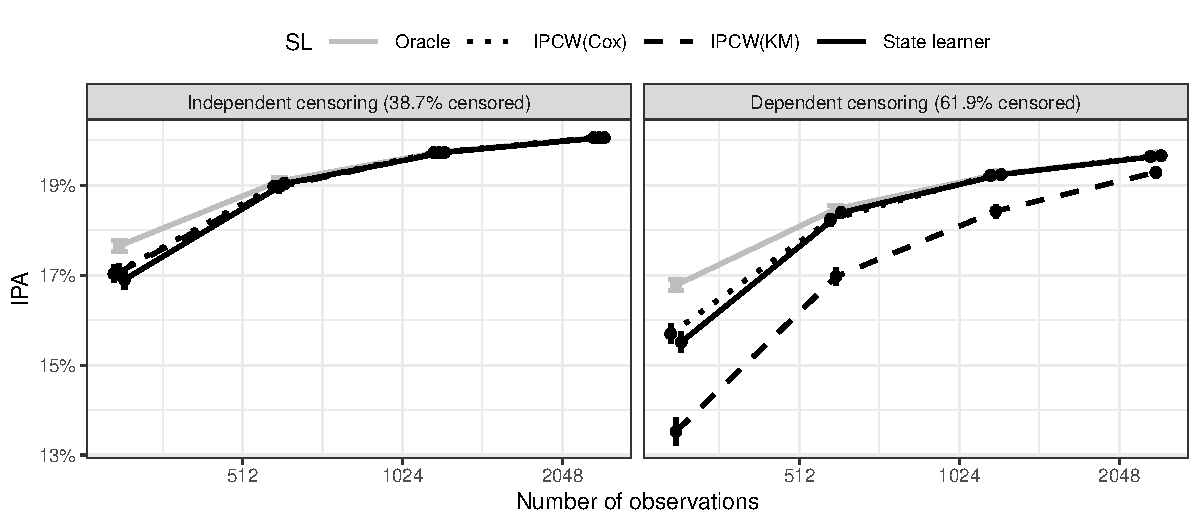
\includegraphics[width=1\linewidth]{experiment-fig-sl-ipcw.pdf}
  \caption[]{For the risk prediction models provided by each of the super
    learners, the IPA is plotted against sample size. The results are averages across 
    1000 simulated data sets and the error bars are used to quantify the Monte Carlo
    uncertainty.
  }
  \label{fig:ipcw-fail}
\end{figure}

We next compare JSSL to the super learner \texttt{survSL}
\citep{westling2021inference}. This is another super learner which
like JSSL works without a pre-specified censoring
model. Note that both JSSL and \texttt{survSL} provide a
prediction model for the event time outcome and also for the
probability of being censored. Hence, we compare the performance of
these methods with respect to both the outcome and the censoring
distribution. Again we use the IPA to quantify the predictive
performance.

The results are shown in Figures~\ref{fig:zelefski-out}
and~\ref{fig:zelefski-cens}. We see that for most sample sizes, JSSL selected prediction models for both censoring and outcome which
have similar or higher IPA compared to the prediction models selected
by \texttt{survSL}.
\begin{figure}
  \centering %
  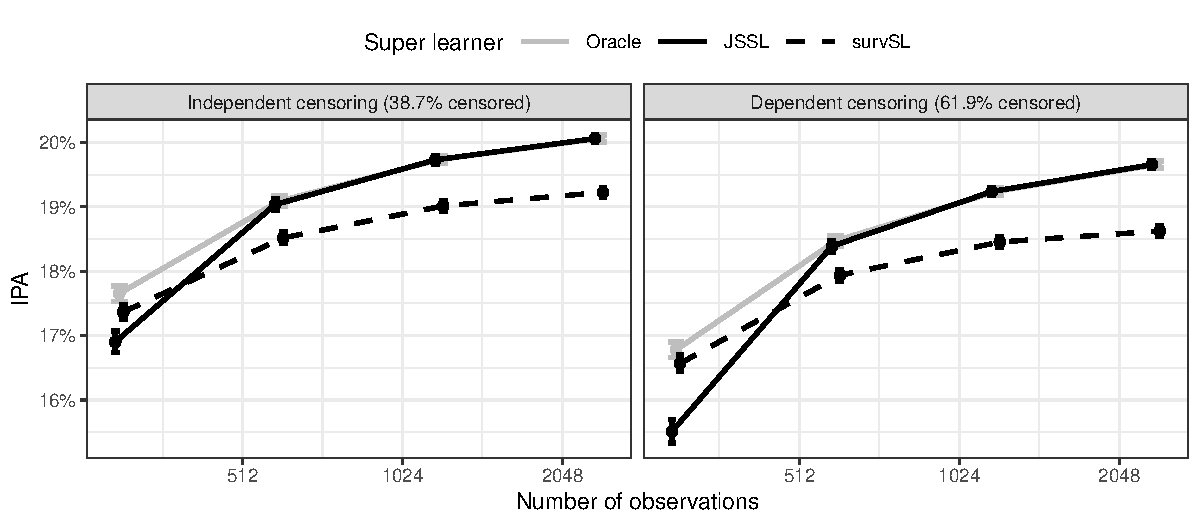
\includegraphics[width=1\linewidth]{experiment-fig-sl-survSL-out.pdf}
  \caption[]{For the risk prediction models of the outcome provided by each
    of the super learners, the IPA at the fixed time horizon is plotted against
    sample size. The results are averages across 1000 repetitions and the error
    bars are used to quantify the Monte Carlo uncertainty.}
  \label{fig:zelefski-out}
\end{figure}

\begin{figure}
  \centering %
  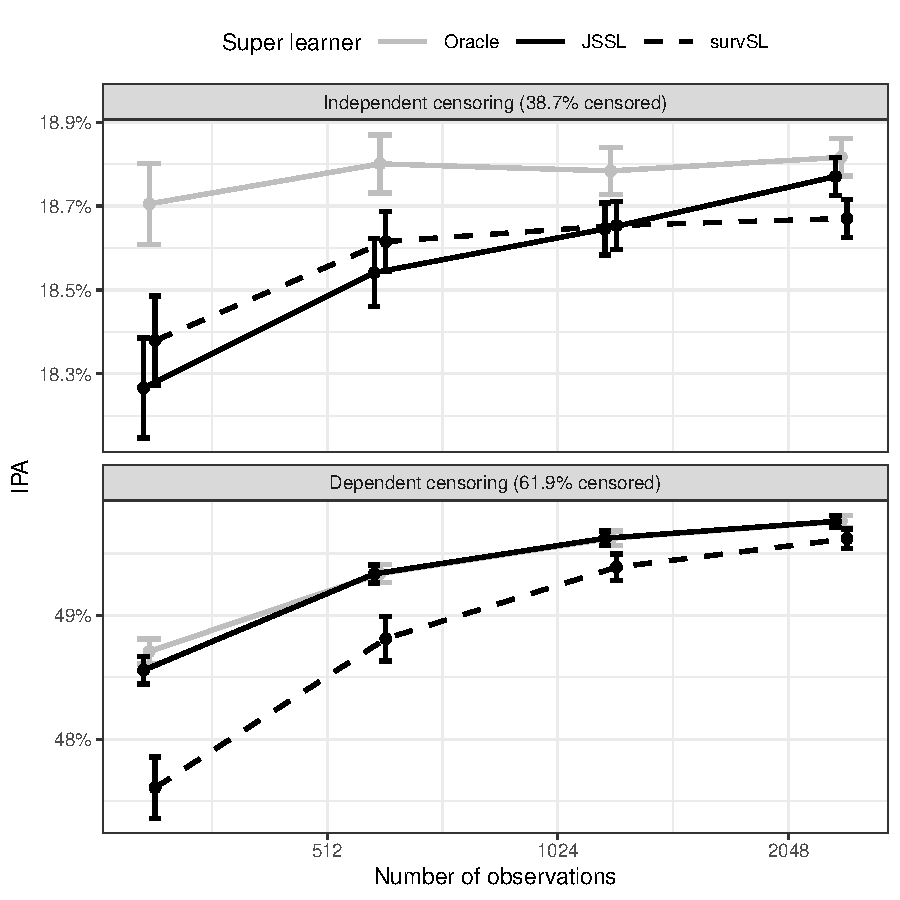
\includegraphics[width=.7\linewidth]{experiment-fig-sl-survSL-cens.pdf}
  \caption[]{For the risk prediction models of the censoring model provided by
    each of the super learners, the IPA at the fixed time horizon is plotted
    against sample size. The results are averages across 1000 repetitions and
    the error bars are used to quantify the Monte Carlo uncertainty.}
  \label{fig:zelefski-cens}
\end{figure}


\section{Prostate cancer study}
\label{sec:real-data-appl}

In this section we use the prostate cancer data of
\cite{kattan2000pretreatment} to illustrate the use of JSSL in the presence of competing risks. We have
introduced the data in Section~\ref{sec:numer-exper}. The data
consists of 1,042 patients who are followed from start of
followup until tumor recurrence, death without tumor
recurrence or end of followup (censored) whatever came first.
We use JSSL to rank libraries of learners for the
cause-specific cumulative hazard functions of tumor
recurrence, death without tumor recurrence, and censoring. The
libraries of learners each include five learners: the
Nelson-Aalen estimator, three Cox regression models
(unpenalized, Lasso, Elastic net) each including additive
effects of the 5 covariates (c.f., Section~\ref{sec:numer-exper}),
and a random survival forest. We use the same set of learners
to learn the cumulative hazard function of tumor recurrence
\( \Lambda_1 \), the cumulative hazard function of death
without tumor recurrence \( \Lambda_2 \), and the cumulative
hazard function of the conditional censoring distribution
$\Gamma$.

This gives a library consisting of \( 5^3 = 125 \) learners for the
conditional state occupation probability function \( F \) defined in
equation~(\ref{eq:F-def}). We use five folds for training and testing
the models, and we repeat training and evaluation five times with
different splits.  The integrated Brier score (defined in
Section~\ref{sec:super-learner-simple}) for all learners are shown in
Figure~\ref{fig:zelefski-real}. We see that the prediction
performance is mostly affected by the choice of learner for the
censoring distribution. Several combinations of learners give similar
performance as measured by the integrated Brier score, as long as a
random forest is used to model the censoring distribution.

\begin{figure}
  \centering %
  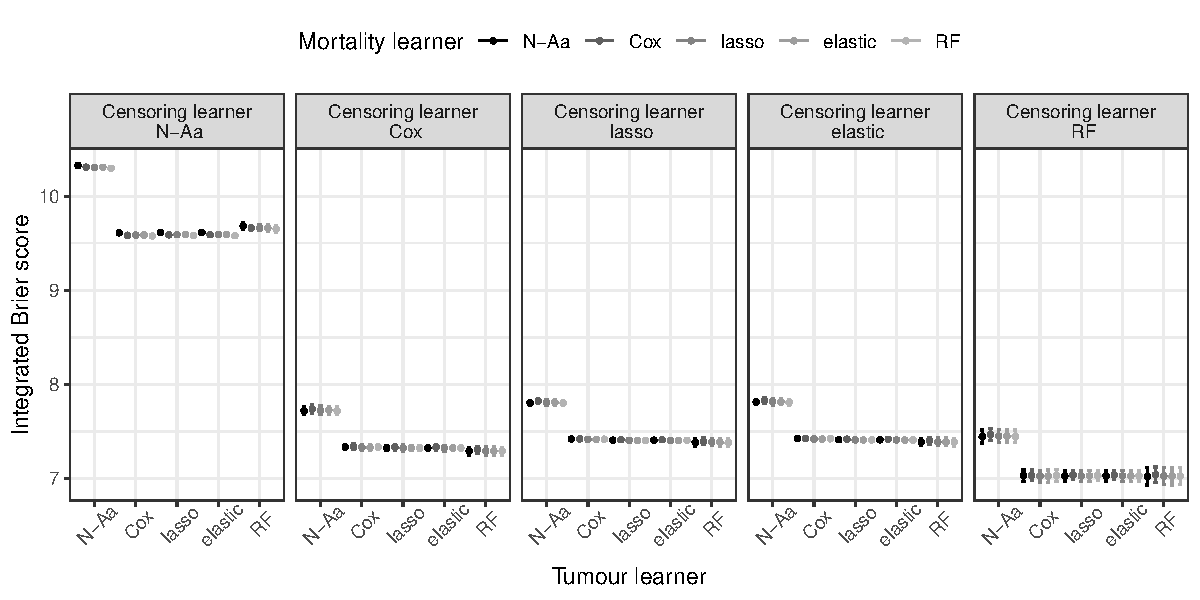
\includegraphics[width=1\linewidth]{real-data-state-learner.pdf}
  \caption[]{The results of applying the 125 combinations of learners to the
    prostate cancer data set. The error bars are based on five repetitions using
    different splits. We refer to learners of \( \Lambda_1 \), \( \Lambda_2 \),
    and $\Gamma$ as `Tumor learner', `Mortality learner', and `Censoring
    learner', respectively.}
  \label{fig:zelefski-real}
\end{figure}


\section{Discussion}
\label{sec:discussion}

The JSSL is a new super learner that can be used with
right-censored data and competing events. Compared to existing
IPCW-based methods, the advantage of JSSL is that
it does not depend on a pre-specified estimator of the
censoring distribution, but selects one automatically based on
a library of candidate learners. Furthermore, JSSL neither requires that the cause-specific cumulative
hazard functions \( \Lambda_j \) can be written as integrals
with respect to Lebesgue measure, nor does it assume a
(semi)parametric formula. In the remainder of this section
we discuss the limitations of our proposal and avenues for
further research.

A major advantage of JSSL is that the performance of each
combination of learners can be estimated without additional nuisance
parameters. A potential drawback of our approach is that we are
evaluating the loss of the learners on the level of the observed data
distribution while the target of the analysis is either the event time
distribution, or the censoring distribution, or both.
Specifically, the finite sample oracle inequality in
Proposition~\ref{prop:oracle-prop} concerns the function \( F \), which
is a feature of \( P \in \mathcal{P} \), while what we are typically
interested in is \( \Lambda_j \) or \( S \), which are features of
\( Q \in \mathcal{Q} \). We emphasise that while JSSL
provides us with estimates of \( \Lambda_j \) and $\Gamma$ based on
libraries \( \mathcal{A}_j \) and \( \mathcal{B} \), the performance
of these learners is not assessed directly for their respective target
parameters, but only indirectly via the performance of \( F \).  For
settings without competing risks, our numerical studies suggest that
measuring the performance of \( F \) also leads to good performance
for estimation of \( S \).

Our proposed super learner can be implemented with a broad library of learners
and using existing software.
% For instance the \texttt{R}-package
% \texttt{riskRegression} \citep{Gerds_Ohlendorff_Ozenne_2023} and the \texttt{R}-package by westling
Furthermore, while
the library \( \mathcal{F}(\mathcal{A}_1,\mathcal{A}_2,\mathcal{B}) \) consists
of \( |\mathcal{A}_1||\mathcal{A}_2||\mathcal{B}| \) many learners, we only need to fit
\( |\mathcal{A}_1| +|\mathcal{A}_2| + |\mathcal{B}| \) many learners in each fold. To
evaluate the performance of each learner we need to perform
\( |\mathcal{A}_1||\mathcal{A}_2||\mathcal{B}| \) many operations to calculate the
integrated Brier score in each hold-out sample, one for each combination of the
fitted models, but these operations are often negligible compared to fitting the
models. Hence JSSL is essentially not more computationally demanding
than any procedure that uses super learning to learn $\Lambda_1$, $\Lambda_2$,
and $\Gamma$ separately. While our proposal is based on constructing the library
\( \mathcal{F} \) from libraries for learning \( \Lambda_1 \), $\Lambda_2$, and
$\Gamma$, it could also be of interest to consider learners that estimate
\( F \) directly.

In our numerical studies, we only considered learners of $\Lambda_j$ and
$\Gamma$ that provide cumulative hazard functions which are piece-wise constant
in the time argument. This simplifies the calculation of \( F \) as the
integrals in equation~(\ref{eq:transition}) reduce to sums. When $\Lambda_j$ or
\( \Gamma \) are absolutely continuous in the time argument, calculating \( F \)
is more involved, but we expect that a good approximation can be achieved by
discretisation.

\subsection{Choice of loss function}
\label{sec:choice-of-loss-function}

Machine learning based on right-censored data
commonly uses the partial log-likelihood as a loss function
\citep[e.g.,][]{li2016regularized,yao2017deep,lee2018deephit,katzman2018deepsurv,gensheimer2019scalable,lee2021boosted,kvamme2021continuous}.
This loss function is also suggested for super learning with
right-censored data by \cite{polley2011-sl-cens}, where data is
assumed to be observed in discrete time. However, the partial
log-likelihood loss does not work well as a measure of performance in
hold-out samples observed in continuous time.  The reason is that the
partial log-likelihood loss assigns an infinite value for any learner
that predicts piece-wise constant cumulative hazard functions when
there are event times in the test set which do not occur in the
learning set.  This problem occurs with prominent survival learners
including the Kaplan-Meier estimator, random survival forests, and
semi-parametric Cox regression models, and these learners cannot be
included in the library of the super learner proposed by
\cite{polley2011-sl-cens}. When a proportional hazards model is
assumed, the baseline hazard function can be profiled out of the
likelihood \citep{cox1972regression}. The cross-validated partial
log-likelihood loss \citep{verweij1993cross} has therefore been
suggested as a loss function for super learning by
\cite{golmakani2020super}.  This choice of loss function restricts the
library of learners to include only Cox proportional hazards models,
and hence excludes many learners such as, e.g., random survival
forests, additive hazards models, and accelerated failure time models.

Alternative approaches for super learning with right-censored
data use an inverse probability of censoring weighted (IPCW)
loss function
\citep{graf1999assessment,van2003unicv,molinaro2004tree,keles2004asymptotically,hothorn2006survival,gerds2006consistent,gonzalez2021stacked},
censoring unbiased transformations
\citep{fan1996local,steingrimsson2019censoring}, or
pseudo-values
\citep{andersen2003generalised,mogensen2013random,sachs2019ensemble}.
All these methods rely on an estimator of the censoring
distribution, and their drawback is that this estimator has to
be pre-specified.

\section*{Conflict of interest}

The authors declare that they have no conflict of interest.


\bibliography{bib.bib}

\appendix

\section{Proofs}
\label{sec:proofs}

This section contains proofs of the results stated in the
paper. Section~\ref{sec:consistency-proof} contains a proof of
the consistency result from Section~\ref{sec:consistency}, and
Section~\ref{sec:oracle-inequalities} contains proofs of the
oracle inequalities from
Section~\ref{sec:finite-sample-oracle}.

\subsection{Consistency}
\label{sec:consistency-proof}

Define
\( \bar{B}_{\tau,P}(F, o) = \bar{B}_{\tau}(F, o) -
\bar{B}_{\tau}(F_P, o) \) and
\( R_{P}(F) = P{[\bar{B}_{\tau,P}(F, \blank)]} \), where the
integrated Brier score \( \bar{B}_{\tau} \) was defined in
Section~\ref{sec:super-learner-simple}. Recall the norm
\( \Vert \blank \Vert_{P}\) defined in
equation~(\ref{eq:norm}).

\begin{lemma}
  \label{lemma:norm}
  \( R_{P}(F) = \Vert F - F_P \Vert_{P}^2 \).
\end{lemma}
\begin{proof}[Proof]
  For any \( t \in [0, \tau] \) and \( l\in \{-1,0,1,2\} \) we have
  \begin{align*}
    & \E_{P}{\left[ (F(t, l, X) - \1{\{\eta(t) = l \}})^2 \right]}
    \\
    & =    \E_{P}{\left[ (F(t, l, X) - F_P(t, l, X) + F_P(t, l, X) - \1{\{\eta(t) = l
      \}})^2 \right]}
    \\
    & =    \E_{P}{\left[ (F(t, l, X) - F_P(t, l, X))^2\right]}
      + \E_{P}{\left[ (F_P(t, l, X) - \1{\{\eta(t) = l \}})^2\right]}
    \\
    & \quad
      + 2\E_{P}{\left[ (F(t, l, X) - F_P(t, l, X))(F_P(t, l, X) - \1{\{\eta(t) = l
      \}})\right]}
    \\
    & =    \E_{P}{\left[ (F(t, l, X) - F_P(t, l, X))^2\right]}
      + \E_{P}{\left[ (F_P(t, l, X) - \1{\{\eta(t) = l \}})^2\right]},
  \end{align*}
  where the last equality follows from the tower property. Hence, using Fubini,
  we have
  \begin{equation*}
    P{[\bar{B}_{\tau}(F, \blank)]}
    = \Vert F - F_P \Vert_{P}^2 + P{[\bar{B}_{\tau}(F_P, \blank)]}.
  \end{equation*}
\end{proof}

\begin{proof}[Proof of Proposition~\ref{prop:stric-prop}]
  The result follows from Lemma~\ref{lemma:norm}.
\end{proof}

\subsection{Oracle inequalities}
\label{sec:oracle-inequalities}

Recall that we use \( \mathcal{F}_n \) to denote a library of learners for the
function \( F \), and that \( \hat{\phi} \) and \( \tilde{\phi} \) denotes,
respectively, the discrete super learner and the oracle learner for the library
\( \mathcal{F}_n \), c.f., Section~\ref{sec:super-learner-simple}.

\begin{proof}[Proof of Proposition~\ref{prop:oracle-prop}]
  First note that minimising the loss \( \bar{B}_{\tau} \) is equivalent to
  minimising the loss \( \bar{B}_{\tau,P} \), so the discrete super learner and
  oracle according to \( \bar{B}_{\tau} \) and \( \bar{B}_{\tau,P} \) are
  identical. By Lemma~\ref{lemma:norm}, \( R_P(F) \geq 0 \) for any
  \( F \in \mathcal{H}_{\mathcal{P}} \), and so using Theorem 2.3 from
  \citep{vaart2006oracle} with \( p=1 \), we have that for all \( \delta >0 \),
\begin{align*}
  & \E_{P}{\left[ R_P(\hat{\phi}_n(\data_n^{-k})) \right]}
  \\
  &  \quad \leq
    (1+2\delta)\E_{P}{\left[ R_P(\tilde{\phi}_n(\data_n^{-k})) \right]}
  \\
  & \qquad + (1+\delta) \frac{16 K}{n}
    \log(1 + |\mathcal{F}_n|)\sup_{F \in \mathcal{H}_{\mathcal{P}}}
    \left\{
    M(F) + \frac{v(F)}{R_P(F)}
    \left(
    \frac{1}{\delta} + 1
    \right)
    \right\}
\end{align*}
where for each \( F \in \mathcal{H}_{\mathcal{P}} \), \( (M(F), v(F)) \) is some Bernstein pair for
the function \(o \mapsto \bar{B}_{\tau,P}(F, o) \). As
\( \bar{B}_{\tau,P}(F, \blank) \) is uniformly bounded by \( \tau \) for any
\( F \in \mathcal{H}_{\mathcal{P}} \), it follows from section 8.1 in \citep{vaart2006oracle} that
\( (\tau, 1.5 P{[\bar{B}_{\tau,P}(F, \blank)^2]}) \) is a Bernstein pair for
\( \bar{B}_{\tau,P}(F, \blank) \). Now, for any \( a,b,c \in \R \) we have
\begin{align*}
  (a-c)^2 - (b-c)^2
  & = (a-b+b-c)^2 - (b-c)^2
  \\
  & = (a-b)^2 + (b-c)^2 +2(b-c)(a-b) - (b-c)^2
  \\
  & = (a-b)
    \left\{
    (a-b) +  2(b-c)
    \right\}
  \\
  & = (a-b)
    \left\{
     a + b -2c
    \right\},
\end{align*}
so using this with \( a=F(t, l, x) \), \( b=F_P(t, l, x) \), and
\( c = \1{\{\eta(t) = l\}} \), we have by Jensen's inequality
\begin{align*}
  & P{[\bar{B}_{\tau,P}(F, \blank)^2]}
  \\
  & \leq
    2\tau\E_{P}{\left[
    \sum_{l=-1}^{2} \int_0^{\tau}
    \left\{
    \left(
    F(t, l, X) - \1{\{\eta(t) = l\}}
    \right)^2
    -
    \left(
    F_P(t, l, X) - \1{\{\eta(t) = l\}}
    \right)^2
    \right\}^2
    \diff t 
    \right]}
  \\
  & =2\tau
    \E_{P}\Bigg[
    \sum_{l=-1}^{2} \int_0^{\tau}
    \left(
    F(t, l, X) - F_P(t, l, X)
    \right)^2
  \\
  & \quad \quad \quad\quad \quad \quad \times
    \left\{
    F(t, l, X) +  F_P(t, l, X)-2 \1{\{\eta(t) = l\}}
    \right\}^2
    \diff t 
    \Bigg]
  \\
  & \leq
    8\tau \E_{P}{\left[
    \sum_{l=-1}^{2} \int_0^{\tau}
    \left(
    F(t, l, X) - F_P(t, l, X)
    \right)^2
    \diff t 
    \right]}.
  \\
  & =
    8\tau \Vert F - F_P \Vert_{P}^2.
\end{align*}
Thus when \( v(F) = 1.5 P{[\bar{B}_{\tau,P}(F, \blank)^2]} \) we have by
Lemma~\ref{lemma:norm}
\begin{equation*}
  \frac{v(F)}{R_P(F)}
  = 1.5 \frac{P{[\bar{B}_{\tau,P}(F, \blank)^2]}}{P{[\bar{B}_{\tau,P}(F, \blank)]}}
  \leq 12 \tau,
\end{equation*}
and so using the Bernstein pairs \( (\tau, 1.5 P{[\bar{B}_{\tau,P}(F, \blank)^2]}) \) we have
\begin{equation*}
  \sup_{F \in \mathcal{H}_{\mathcal{P}}}
  \left\{
    M(F) + \frac{v(F)}{R_P(F)}
    \left(
      \frac{1}{\delta} + 1
    \right)
  \right\}
  \leq \tau
  \left(
    13 + \frac{12}{\delta}
  \right).
\end{equation*}
For all $\delta>0$ we thus have
\begin{align*}
  \E_{P}{\left[ R_P(\hat{\phi}_n(\data_n^{-k})) \right]}
  \leq
  &(1+2\delta)\E_{P}{\left[ R_P(\tilde{\phi}_n(\data_n^{-k})) \right]}
  \\
  & \quad
    + (1+\delta)\log(1 + |\mathcal{F}_n|) \tau \frac{16 K}{n}
    \left(
    13 + \frac{12}{\delta}
    \right),
\end{align*}
and then the final result follows from Lemma~\ref{lemma:norm}.
\end{proof}

\begin{proof}[Proof of Corollary~\ref{cor:asymp-cons}]
  By definition of the oracle and Lemma~\ref{lemma:norm},
  \begin{equation*}
    \E_{P}{\left[ \Vert \tilde{\phi}_n(\data_n^{-k}) - F_P \Vert_{P}^2
      \right]} \leq \E_{P}{\left[ \Vert \phi_n(\data_n^{-k}) - F_P \Vert_{P}^2
      \right]}  
  \end{equation*}
  for all \( n \in \N \). The results then follows from
  Proposition~\ref{prop:oracle-prop}.
\end{proof}


\end{document}
% end of file template.tex

